\documentclass[12pt]{article}
\usepackage{graphicx,epsfig,palatino,epstopdf}


\title{Lab 1: EKF}
\author{
        Miquel Marti Rabadan\\
        miquelmr@kth.se
}
\date{\today}



\begin{document}
\maketitle

%\begin{abstract}
%This is the paper's abstract \ldots
%\end{abstract}

%\section{Introduction}
%This is time for all good men to come to the aid of their party!

\section{PART I - Preparatory Questions}
\subsection{Linear Kalman Filter:}
\paragraph{1 - What is the difference between a 'control' \(u_t\), a 'measurement' \(z_t\) and the
state \(x_t\). Give examples of each.} 
Control data \(u_t\) is used in the predict phase to get current state vector \(x_t\), together with  previous state vector \(x_{t-1}\), so that current state is a function of both: \(x_t=g(u_t,x_{t-1})\). Measurement is instead used in update phase and is a function of the current state vector \(x_t\). In the example in the book with the robot and the door the control is the action that the robot does (opening the door or not), the state is if the door is open or closed and the measurement the reading of this last by the robot sensors. "z refined version of current state, u how state changes"
\paragraph{2 - Can the uncertainty in the belief increase during an update? Why (or not)?}
It cannot increase. Looking at the update step using the information matrix (inverse of the uncertainty matrix), we see that the information can only grow as it is the predicted information matrix plus the term \( C^T_tR_t^{-1}C_t\)which is positive semidefinite as \(R_t\) is the covariance matrix of the noise. As the uncertainty is the inverse, can only decrease.
\paragraph{3 - During update what is it that decides the weighting between measurements and belief?}
A term called \textit{Kalman gain}, which is related to the ratio between the measurement error covariance and the  uncertainty matrix.
\paragraph{4 - What would be the result of using a too large a covariance (Q matrix) for the measurement model?}
The measurement error covariance would be big so the Kalman gain would be small and the updated mean and uncertainty would just approach the same value they had before, making the update slower and in the limit avoiding any update.
\paragraph{5 - What would give the measurements an increased effect on the updated state estimate?}
A larger Kalman gain, so a small covariance matrix for the measurement error model.
\paragraph{6 - What happens to the belief uncertainty during prediction? How can you show that?}
Belief uncertainty often grows as it is defined as \(\bar{\Sigma}_t=Q_t+A_t\Sigma_{t-1}A_t^T\) with \(Q_t\) being positive definite and the second term being usually bigger than \(\Sigma\) for \(A\) matrix of real systems being \(A \geq I\).
\paragraph{7 - How can we say that the Kalman filter is the optimal and minimum least square error estimator in the case of independent Gaussian noise and Gaussian priori distribution?}
It gives the true posterior distribution for a linear Gaussian system. If one tries to derive a \(mu\) which has lower expected square error than the Gaussian mean, arrives to the conclusion that the Gaussian mean equals this one, so it is the optimal.
\paragraph{8 - In the case of Gaussian white noise and Gaussian priori distribution, is
the Kalman Filter a MLE and/or MAP estimator?}
Assuming the initial state has a Gaussian distribution, it can be considered as a prior for the estimation of the next state, so it is a MAP estimator. If no prior is used then the mean is the MLE of the Gaussian posterior, the maximum of the bell shape.
\subsection{Extended Kalman Filter:}
\paragraph{9 - How does the extended Kalman filter relate to the Kalman filter?}
It is a Kalman filter of a linearised system.
\paragraph{10 - Is the EKF guaranteed to converge to a consistent solution?}
No, the update depends on the previous estimate and an estimate implied by linearising the measurement function, if this linearisation is far from \(\mu_z\), the measurement does not really imply \(\mu_z\) and the updated state can be moved to an unreal one. Therefore, the consistency depends on the significance of the nonlinearity where the function has been linearised.
\paragraph{11 - If our filter seems to diverge often can we change any parameter to try
and reduce this?}
We can replace \(\mu_z\) by a state \(\tilde{\mu}\) which lies along the line between \(\mu_z\) and \(\bar{\mu}_t\) which minimizes the error between the measurement \(z_t\) and the function of this new state, providing better consistency. We can increase the relative size of the measurement covariance, as divergence occurs most likely on update phase. If instead it is due to a poor data association, the matching threshold can be changed.

\subsection{Localization:}

\paragraph{12 - If a robot is completely unsure of its location and measures the range r
to a know landmark with Gaussian noise what does its posterior belief of
its location p(x, y, \(\theta|\)r) look like? So a formula is not needed but describe
it at least.} It will know that it is at a distance r of the landmark but will not know in which direction, so all directions will be as likely, giving a circle of uniform probability at distance r of the landmark. Due to the Gaussian noise on the measurement of r, this circle will  become a donut with Gaussian distribution on the radial axis and uniform distribution on the angular.

\paragraph{13 - If the above measurement also included a bearing how would the posterior
look?}
Then the angle would also be estimated and would be Gaussian, so it would be a Gaussian distribution in both radial and angular axis.

\paragraph{14 - If the robot moves with relatively good motion estimation (prediction error
is small) but a large initial uncertainty in heading \(\theta\) how will the posterior
look after travelling a long distance without seeing any features?}
It would have an arc shape, so the distance from the starting point is properly estimated, but the heading was not so it can take any value and the final position can be any on the arc at the distance travelled.

\paragraph{15 - If the above robot then sees a point feature and measures range and bearing to it how might the EKF update go wrong?}
The Jacobian used for linearization in the update phase of the direction will produce an update that is a straight line, which will not coincide with the arc mentioned before. The Gaussian will not be curved along the arc so the update can diverge easily.

\section{PART II}
\subsection{Warm up problem with Standard Kalman Filter}
\paragraph{1 - What are the dimensions of \(\epsilon_k\) and \(\delta_k\)? What parameters do you need to define in order to uniquely characterize a white Gaussian?}
The vector \(\epsilon_k\) has two elements as it has to have the same as \(x_k\) and \(\delta_k\) has one element as \(Cx_k\) gives one element. To characterize a white Gaussian you need to define the mean and the covariance matrix. In the case of \(delta_k\) the mean and the variance are just one value, while for \(\epsilon_k\) the mean is a vector of two elements and the covariance matrix has size 2x2.
\paragraph{2 - Make a table showing the roles/usages of the variables(x, xhat, P, G, D, Q, R, wStdP, wStdV, vStd, u, PP). To do this one must go beyond simply reading the comments in the code to seeing how the variable is used. (hint some of these are our estimation model and some are for simulating the car motion).}
Table \ref{tab:vars} shows the roles/usages of the mentioned variables.
\begin{table}[]
\centering
\caption{Variables and their roles/usages \label{tab:vars}}
\label{my-label}
\begin{tabular}{l | p{5cm}}
\textbf{Variable name} & \textbf{Role/Usage} \\\hline
x                      & True state vector, composed by two elements: position and velocity	.                    \\
xhat                   & Estimated state vector.\\
P                      & Belief uncertainty matrix after prediction.                    \\
G                      & Noise model matrix in prediction phase, here just identity matrix.\\
D                      & Noise model matrix in update phase, here just 1x1 identity matrix.                    \\
Q                      & Uncertainty/covariance matrix of noise in the measurement model (1x1 matrix as has only one element).                    \\
R                      & Uncertainty/covariance matrix of process noise used in the process phase.\\
wStdP                  & Standard deviation of noise on simulated position update.\\
wStdV                  & Standard deviation of noise on simulated velocity update.\\
vStd                   & Standard deviation of measurement noise on simulated position.\\
u                      & "Control" signal used in prediction phase and for the simulation.                     \\
PP                     & Belief uncertainty matrix record, each record has the 4 elements in the original matrix in a vector.                   
\end{tabular}
\end{table}

\paragraph{3 - Please answer this question with one paragraph of text that summarizes broadly what you learn/deduce from changing the parameters in the code as described below. Choose two illustrative sets of plots to include as demonstration. What do you expect if you increase/decrease the covariance matrix of the modelled (not the actual simulated) process noise/measurement noise 100 times(one change in the default parameters each time) for the same underlying system? Characterize your expectations. Confirm your expectations using the code (save the corresponding figures so you can analyse them in your report). Do the same analysis for the case of increasing/decreasing both parameters by the same factor at the same time. (Hint: It is the mean and covariance behaviour over time that we are asking about.)}
We expect that if the measurement noise variance increases, the estimates will be pessimistic or conservative so convergence will be slower. This also produces that the covariance does not tend to zero  as the data association is ambiguous. If by the contrary they decrease, the measurement will have an increased effect on the updated state estimate, which can be seen as optimistic as the measurement is considered to be more reliable because it is less noisy, and the covariance in the final state estimate error converges to a value closer to zero, though the variance of the error in velocity estimation over time increases considerably as it prevents the mean to move to a better estimate.
If we increase the noise variance for the process model the error covariance converges to value closer to zero for the position, but not for the speed and the variance of the error in velocity estimation over time increases considerably. If instead we decrease it, the estimation error covariance of both converges to zero. Figures \ref{fig:q3_g} and \ref{fig:q3_l} show the position and speed estimates against the true value and the estimated error covariances when increasing/decreasing both noise covariance matrix values.
Increasing both noise variances, the covariances of the estimated error do not converge to zero for any of the state variables (pessimistic). Decreasing both noise variances, both converge to zero and faster (optimistic).

\begin{figure}[htbp]
 \centering
 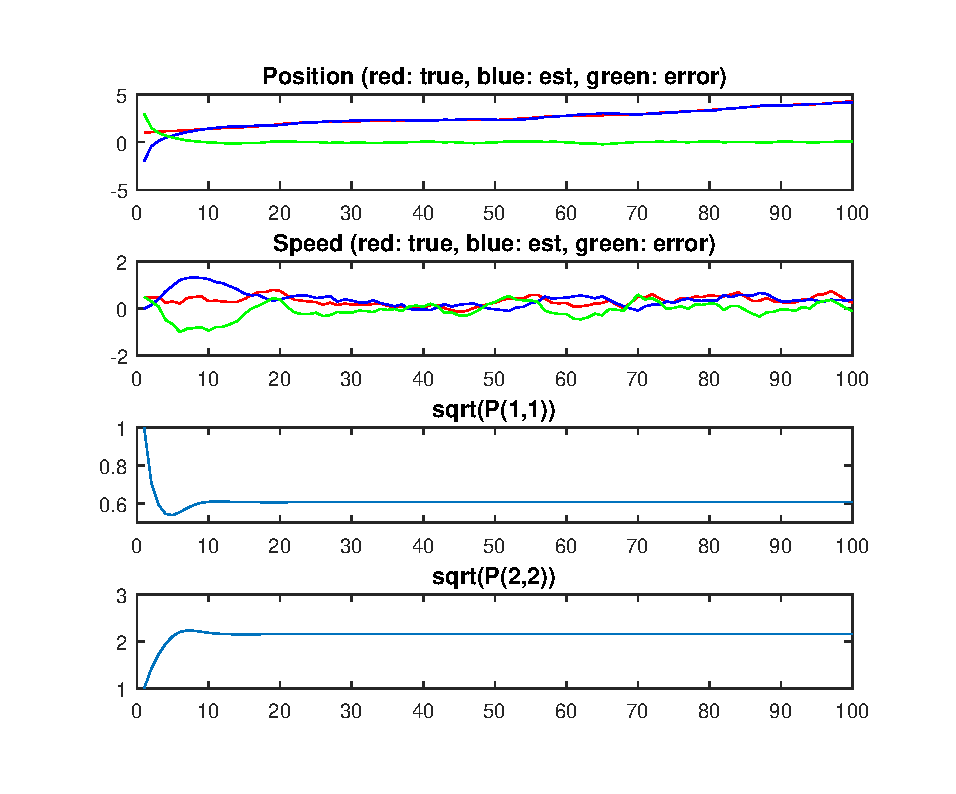
\includegraphics[width=\textwidth]{q3_g}
 \caption{Position and speed estimates against true values and estimated error covariances for \(R'=100R\).}
 \label{fig:q3_g}
\end{figure}

\begin{figure}[htbp]
 \centering
 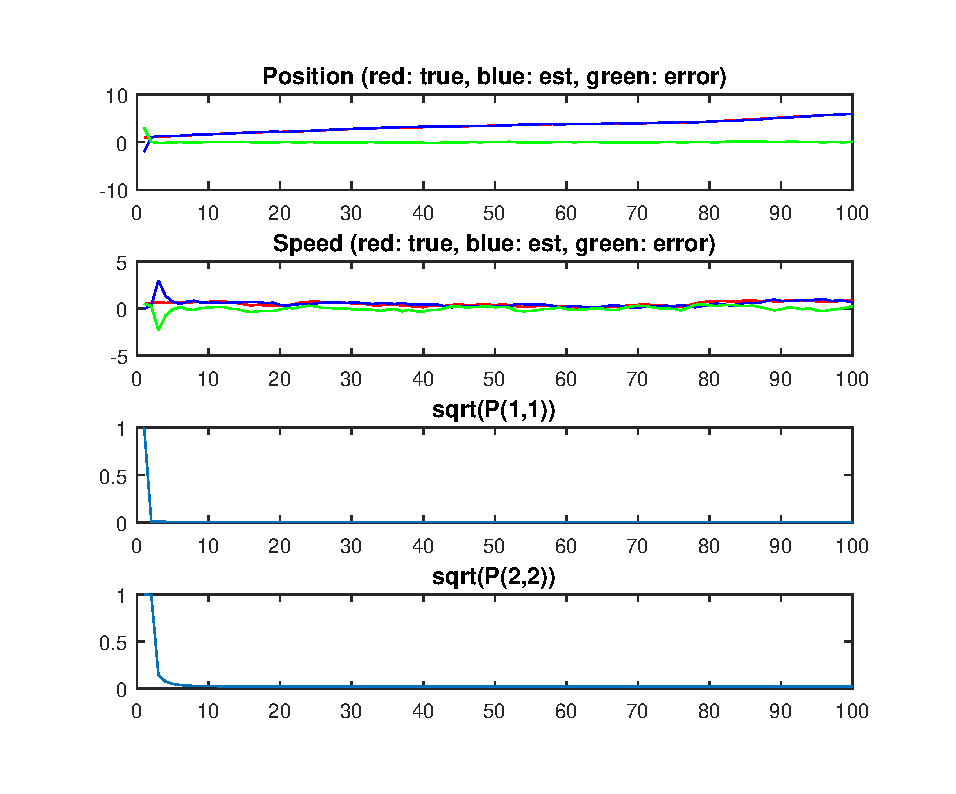
\includegraphics[width=\textwidth]{q3_l}
 \caption{Position and speed estimates against true values and estimated error covariances for \(R'=\frac{R}{100}\).}
 \label{fig:q3_l}
\end{figure}

\paragraph{4 - How do the initial values for P and xhat affect the rate of convergence and the error of the estimates (try both much bigger and much smaller)}
Making P much bigger has similar effect to making covariances of noise in process model smaller, increasing the relative size between P and R, which makes the Kalman gain bigger for the first iteration and thus makes it converge faster but is after that sensitive to the noise in the process. Making it smaller makes the covariance of the error converges slower to a non-zero value but the mean converges to zero.

\subsection{Main problem: EKF Localization}

\paragraph{5 - Which parts of (2) and (3) are responsible for prediction and update steps?}
For the prediction step the second equation in (3) is the responsible, \(\bar{bel}(\textbf{x}_t)\). For the update step, the first equation in (3), \(bel(\textbf{x}_t)\). The third equation defines the initial belief used in the first prediction step.
	
\paragraph{6 - In the maximum likelihood data association, we assumed that the measurements are independent of each other. Is this a valid assumption? Explain why.}
It is not valid in general if the landmarks map is static as for example if you move along a would subsequent measurements will be seeing this same wall. It would hold better in a non-static environment where objects move randomly across the map. It is though conditionally independent given a map and a position if the noises of the different measurements are independent.

\paragraph{7 - What are the bounds for \(\delta_M\)  in (8)? How does the choice of \(\delta_M\) affect the outlier rejection process? What value do you suggest for \(\lambda_M\) when we have reliable measurements all arising from features in our map, that is all our measurements come from features on our map? What about a scenario with unreliable measurements with many arising from so called clutter or spurious measurements?}
\(\delta_M\) can take values between 0 and 1 as it is a probability. 
A high value would give a threshold for the Mahalanobis distance defining regions so far that the probability of being in that region  is very small, \(1-\delta_M\), If there are many expected outliers, our scenario includes unreliable measurements, \(\delta_M\) should be smaller so the outliers are rejected, if we expect no outliers because we have reliable measurements from features on our map \(\delta_M\) would approach 1. That means \(\lambda_M\) big when we expect few outliers or none, and smaller when there are many unreliable measurements.


\paragraph{8 - Can you think of some down-sides of the sequential update approach(Alg 3)? Hint: How does the first [noisy] measurements affect the intermediate results?}
In the sequential update the association of the \(i^{th}\) measurement is computed using estimates updated using the the \((i-1)^{th}\) measurement. If the previous is noisy or an outlier, the next will depend on this error as will be computed from an erroneous estimate. The sequential update algorithm is sensitive to noise and outliers.

\paragraph{9 - How can you modify Alg 4 to avoid redundant re-computations?}
Exploiting the symmetries in the covariances and uncertainties matrices.


\paragraph{10 - What are the dimensions of \(\hat{\upsilon}_t\) and \(\hat{H}_t\) in Alg 4? What were the corresponding dimensions in the sequential update algorithm? What does this tell you?}
\(\hat{\upsilon}_t\) is a vector with length MN, being N the number of observations and M the length of the measurement vector. In the sequential update algorithm it was a vector of the same length as the state and measurement vector. \(\hat{H}_t\) has size MNxP, P being the length of the state vector. Before it had size MxP. This tells that the computation cost will be much higher.

\subsection{Data sets}
\subsubsection*{map\_o3+so\_o3\_ie}
Results for first test scenario.

\begin{verbatim}
mean error(x, y, theta)=(0.000275, 0.000601, -0.004150)
mean absolute error=(0.004191, 0.005330, 0.036612)
total_time =79.123365
\end{verbatim}

\begin{figure}[htbp]
 \centering
 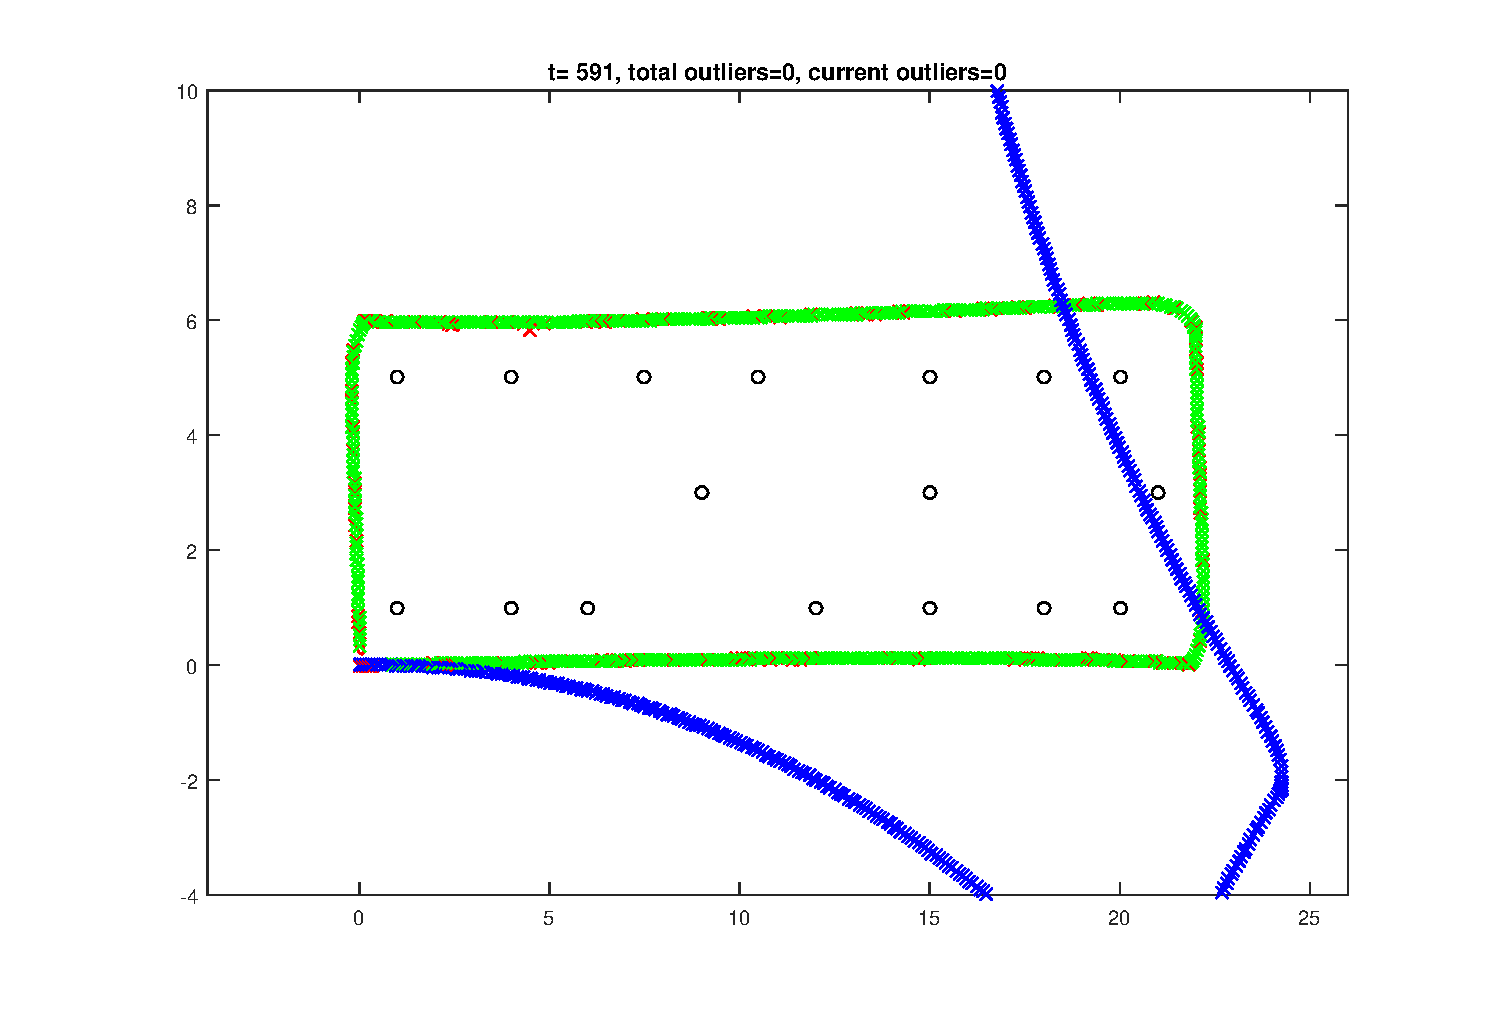
\includegraphics[width=\textwidth]{test1_fig1}
 \caption{Estimated map and movement 1st scenario.}
\end{figure}

\begin{figure}[htbp]
 \centering
 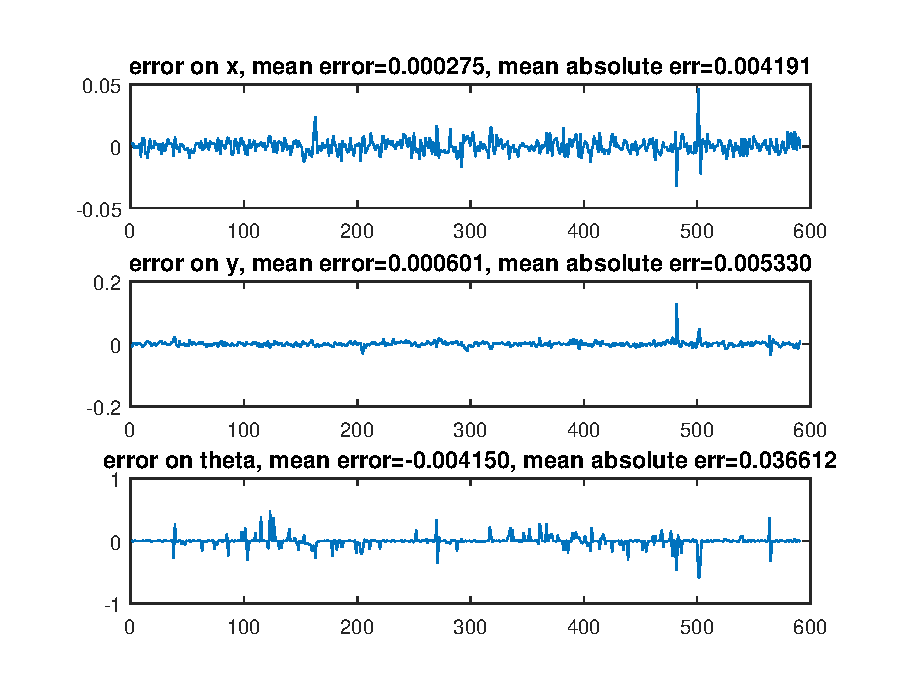
\includegraphics[width=\textwidth]{test1_fig2}
 \caption{Estimated map and movement 1st scenario.}
\end{figure}
\begin{figure}[htbp]
 \centering
 \includegraphics[width=\textwidth]{test1_fig3}
 \caption{Estimated map and movement 1st scenario.}
\end{figure}



\subsubsection*{map\_pent\_big\_10+so\_pb\_10\_outlier}
Results for second scenario with \(R=diag([0.01,0.01,0.01]);\) and \(Q=diag([0.2,0.2]).^2\):
\begin{verbatim}
mean error(x, y, theta)=(0.004337, 0.008119, -0.008135)
mean absolute error=(0.089515, 0.091673, 0.072631)
total_time =437.085723
\end{verbatim}
\begin{figure}[htbp]
 \centering
 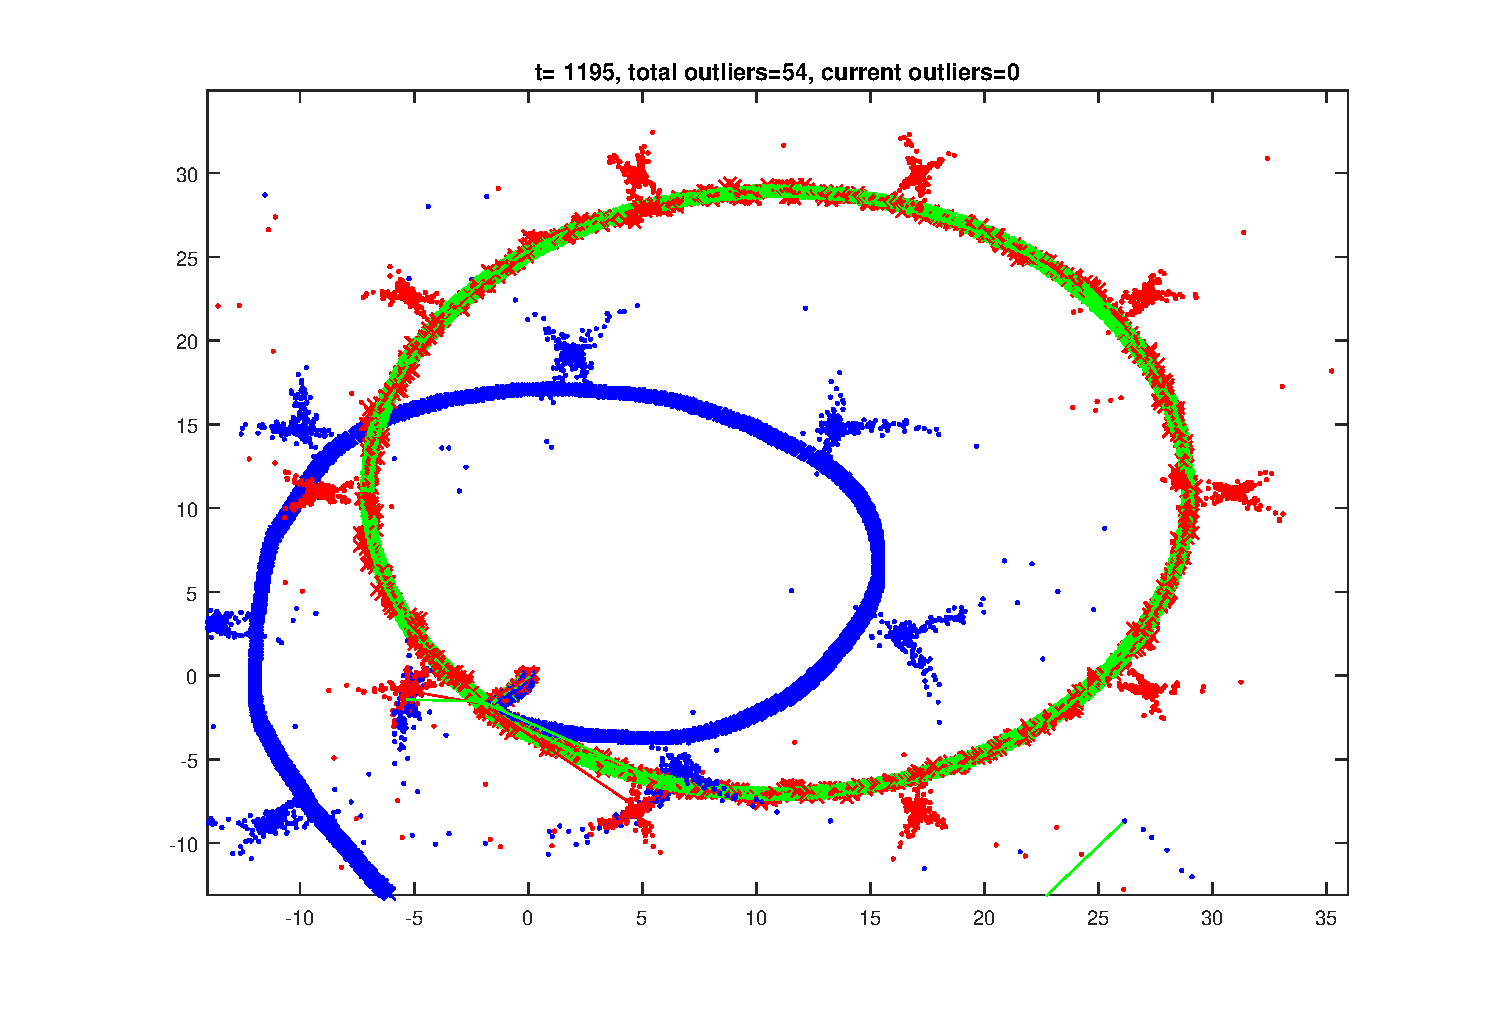
\includegraphics[width=\textwidth]{test2_fig1}
 \caption{Estimated map and movement 2nd scenario.}
\end{figure}

\begin{figure}[htbp]
 \centering
 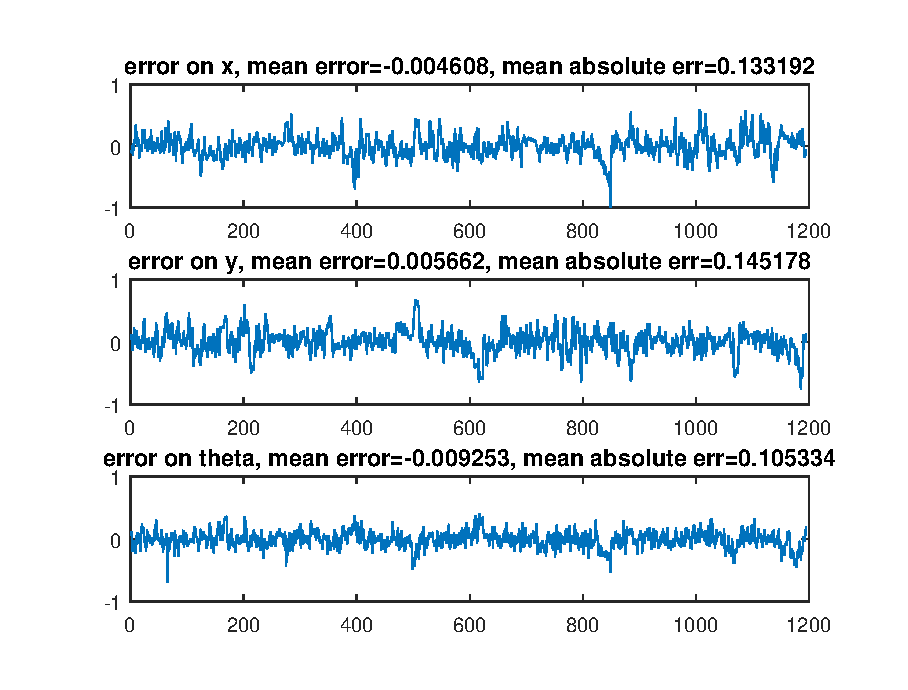
\includegraphics[width=\textwidth]{test2_fig2}
 \caption{Error over time.}
\end{figure}
\begin{figure}[htbp]
 \centering
 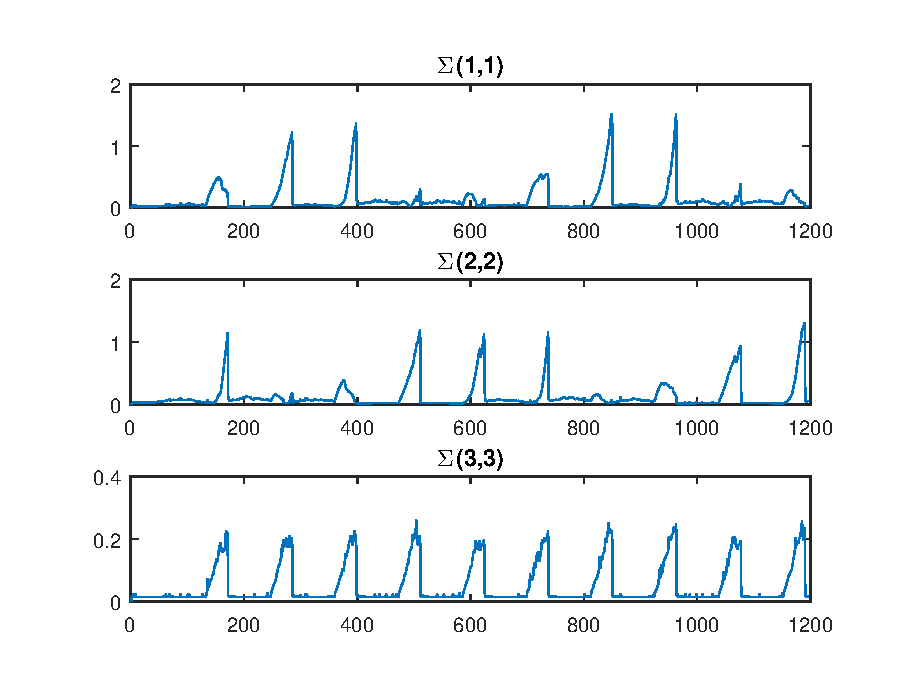
\includegraphics[width=\textwidth]{test2_fig3}
 \caption{Uncertainty over time.}
\end{figure}

\subsubsection*{map\_pent\_big\_40+so\_pb\_40\_no}
Results for third scenario with \(R=diag([1,1,1]);\) and \(Q=diag([0.1,0.1]).^2\) with sequential update:

\begin{verbatim}
mean error(x, y, theta)=(-2.618506, -1.733604, 0.439642)
mean absolute error=(4.462436, 4.795607, 0.440101)
total_time =35.826410
\end{verbatim}

\begin{figure}[htbp]
 \centering
 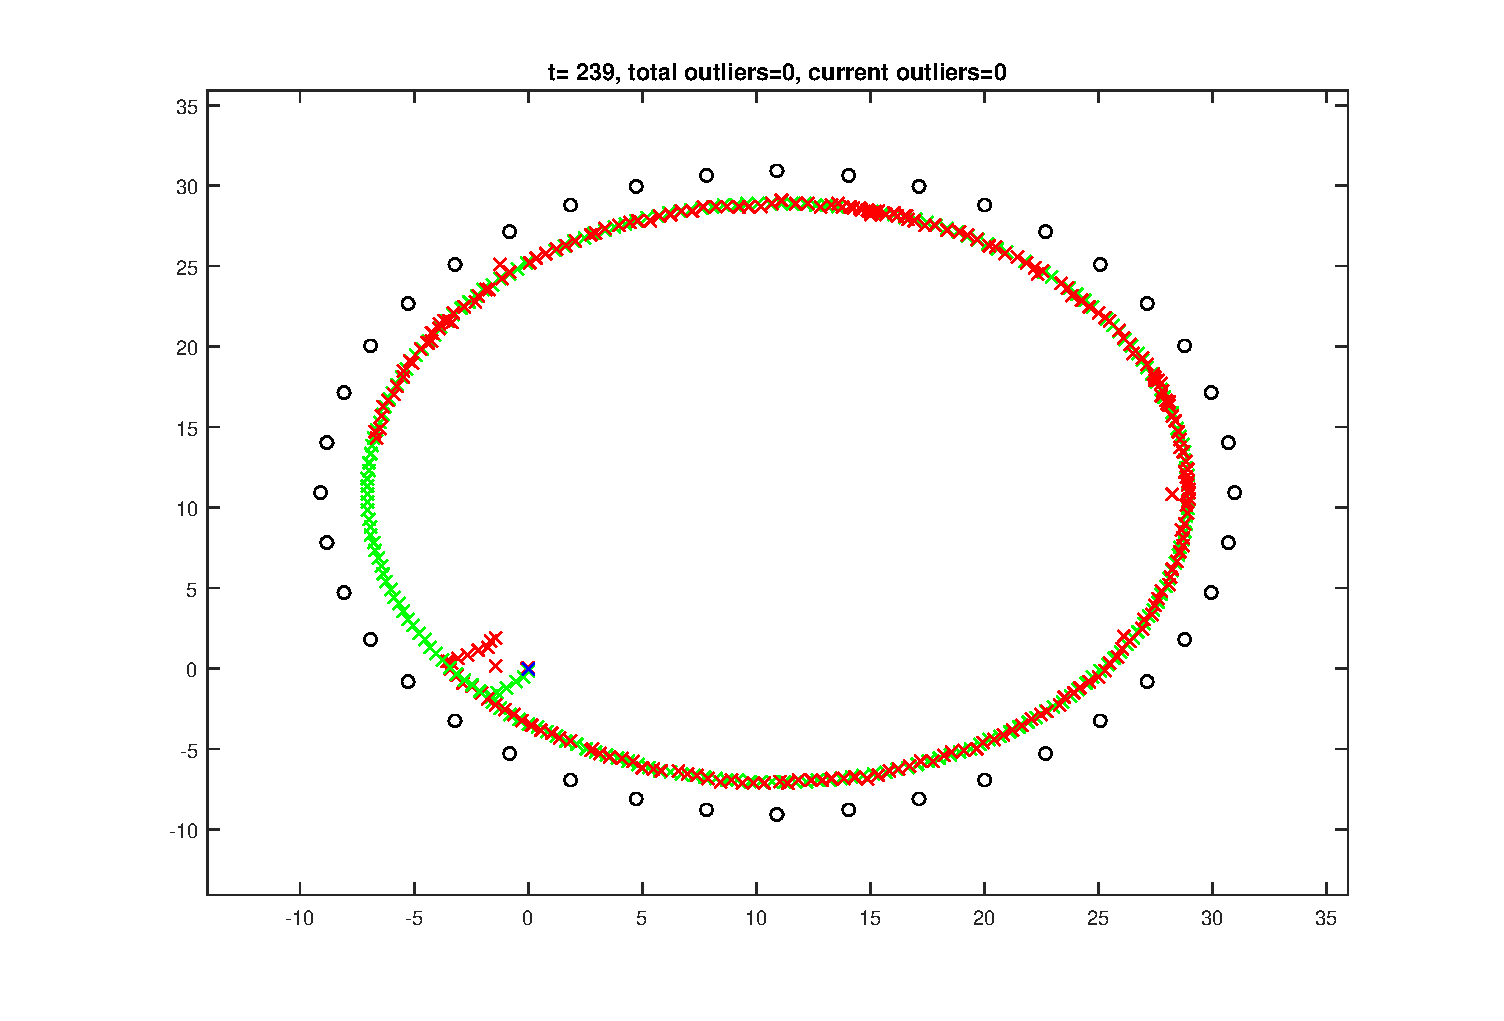
\includegraphics[width=\textwidth]{test3_fig1}
 \caption{Estimated map and movement 3rd scenario.}
\end{figure}

\begin{figure}[htbp]
 \centering
 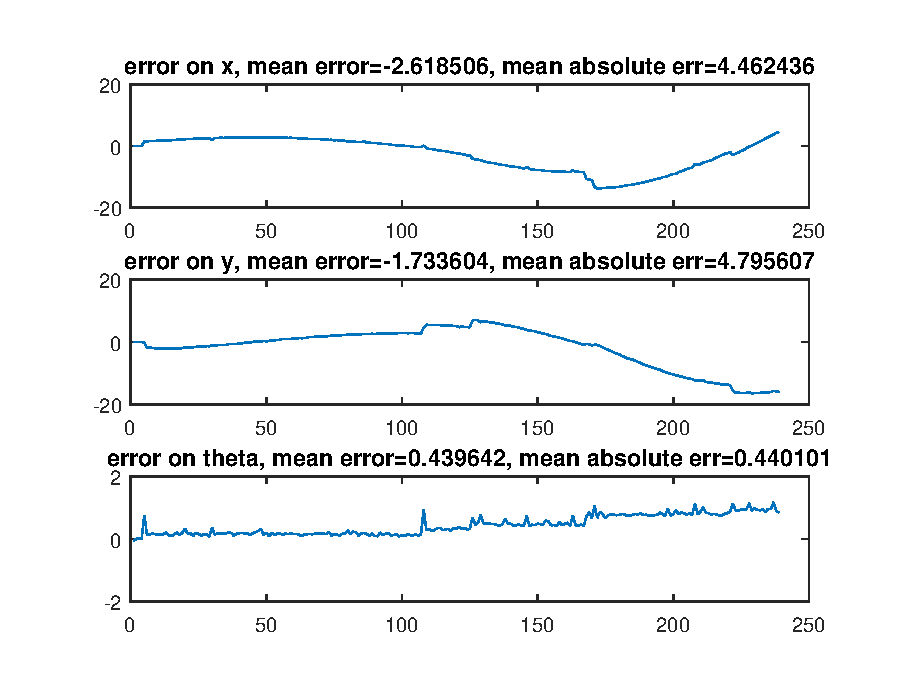
\includegraphics[width=\textwidth]{test3_fig2}
 \caption{Error over time.}
\end{figure}
\begin{figure}[htbp]
 \centering
 \includegraphics[width=\textwidth]{test3_fig3}
 \caption{Uncertainty over time.}
\end{figure}

	Results for third scenario with \(R=diag([1,1,1])\) and \(Q=diag([0.1,0.1]).^2\) with batch update:
\begin{verbatim}
mean error(x, y, theta)=(-0.026019, -0.022660, 0.018390)
mean absolute error=(0.080351, 0.088318, 0.047883)
total_time =27.928715
\end{verbatim}
\begin{figure}[htbp]
 \centering
 \includegraphics[width=\textwidth]{test4_fig1}
 \caption{Estimated map and movement 3rd scenario.}
\end{figure}

\begin{figure}[htbp]
 \centering
 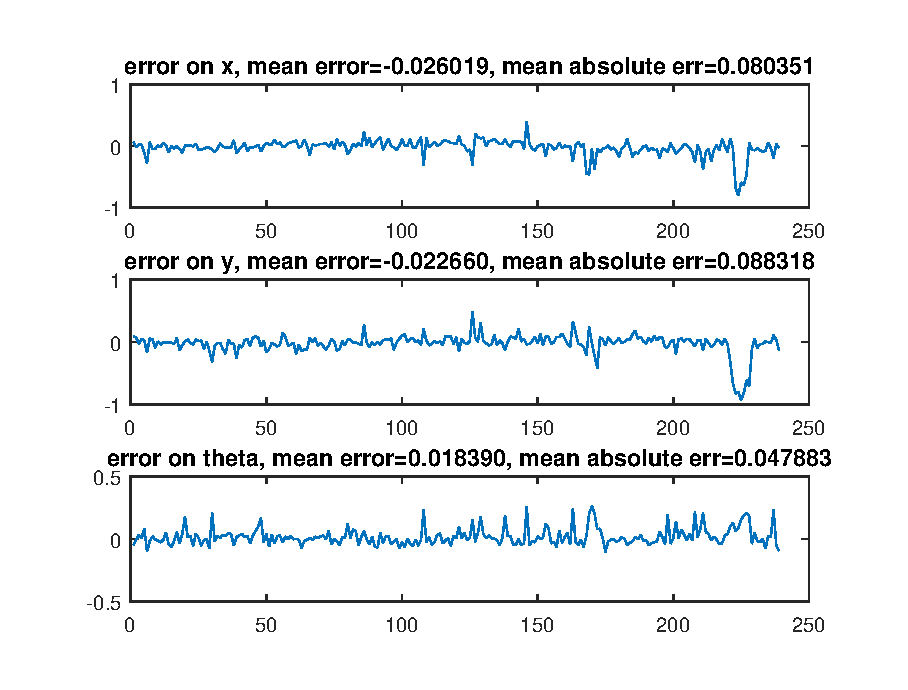
\includegraphics[width=\textwidth]{test4_fig2}
 \caption{Error over time.}
\end{figure}
\begin{figure}[htbp]
 \centering
 \includegraphics[width=\textwidth]{test4_fig3}
 \caption{Uncertainty over time.}
\end{figure}








%\section{Previous work}\label{previous work}
%A much longer \LaTeXe{} example was written by Gil~\cite{Gil:02}.
%
%\section{Results}\label{results}
%In this section we describe the results.
%
%\section{Conclusions}\label{conclusions}
%We worked hard, and achieved very little

\end{document}
This is never printed
